\subsection*{1.1}
%1. Build the circuit shown below using BS170 transistor and a resistor RD = 470 . %Supply
%voltage is VDD = +15 V. Transistor gate is connected to a variable power supply.   
The circuit in figure 1 was built using the NI Elvis experimental setup using a drain resistor, $R_D$ measured as $462 \Omega$.

    %FIG1 CIRCUIT DIAGRAM OF A HALFWAVE RECTIFIER
    \begin{figure}[h!]
        \centering
        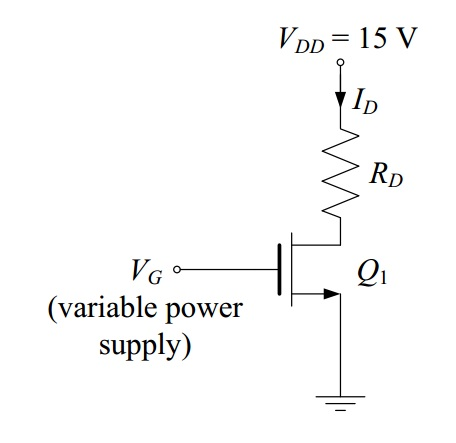
\includegraphics[width=6cm]{circuit_task_1.jpg}
        \captionof{figure}{The circuit in Task 1}
    \end{figure}

\subsection*{1.2}
% 2. Determine the threshold voltage and the transconductance parameter k of the MOS
%transistor. 
%In particular, find the voltage VT for which noticeable drain current appears,
The threshold voltage was determined by observing the drain current while increasing the voltage at the gate. The drain current, $I_{D_0}$ was found be observing the voltage drop over the resistor $R_D$: $$I_{D_0} = \dfrac{V_{DD}-V_D}{R_D} = \dfrac{15.373 - V_D}{462 \ \Omega}$$ 

Table 1 shows the results of these calculation for increasing gate voltage. 

\pagebreak

   \begin{table}[htbp]
     \centering
     \caption{Data for the gate voltage versus drain current}
       \begin{tabular}{cc}
       $V_{G_0}$ [V]       & $I_{D_0}$ [mA] \\
       0.0          & 0.000 \\
       0.2          & 0.000 \\
       0.4          & 0.000 \\
       0.6          & 0.000 \\
       0.8          & 0.000 \\
       1.0          & 0.000 \\
       1.2          & 0.000 \\
       1.4          & 0.000 \\
       1.6          & 0.000 \\
       1.7          & 0.310 \\
       1.8          & 0.903 \\
       1.9          & 2.312 \\
       2.0          & 5.526 \\
       2.1          & 10.331 \\
       2.2          & 17.474 \\
       2.3          & 25.872 \\
       2.4          & 32.344 \\

       \end{tabular}%
     \label{tab:addlabel}%
   \end{table}%
The threshold voltage was determined at the point where an increase of the gate voltage caused a significant change in the drain current, around 0.5 mA. The threshold voltage was determined by doing a polynomial fit (in Matlab, see appendix 1) to the data collected and an exact value found to be be $V_T = 1.74 \ V$.


The transconductance factor was estimated by taking one point from the graph when $V_G > V_T$. The point chosen was $I_{D_0}  = 10.331 \ mA  \approx 10 \ mA$ and corresponding gate voltage is $V_{G_0} = 2.1 \ V$. Therefore: $$ k = \dfrac{I_{D_0}}{(V_{G_0}-V_T)^2} = \dfrac{9.255 \ mA}{(2.1 \ V - 1.74 \ V)^2} = 79.7 \ \dfrac{mA}{V^2} $$

\begin{figure}[h!]
        \centering
        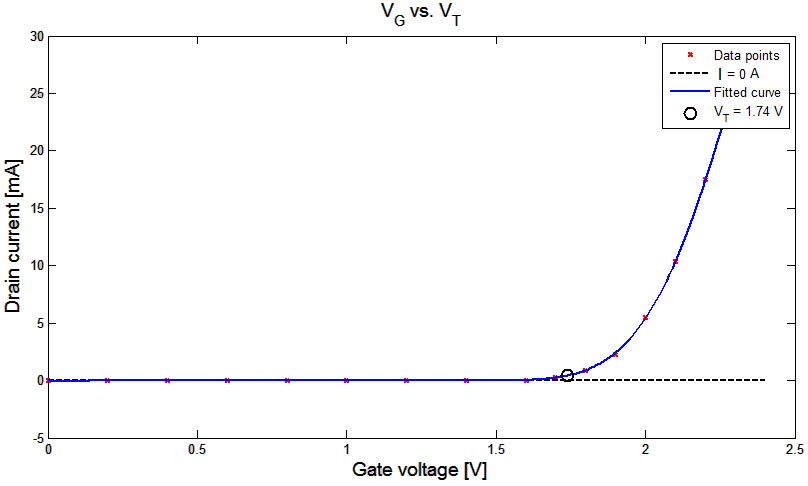
\includegraphics[width=16cm]{Task1_matlab.png}
        \captionof{figure}{Plot of the drain current versus the gate voltage ($I_D$ vs. $V_G$)}
\end{figure}

%This data can also be estimated by measuring the voltage over $R_D$ and then calculating $I_D = \dfrac{V_{DD}-V_D}{R_D}$ as suggested in the assignment. This gives the same results as measuring the current as done here above.

%Note that the parameter k here includes W/L and 0.5 factor
%that you have in the drain current formula ID = 0.5 kn’W/L(VGS–VT)2, i.e., k = 0.5kn’W/L.
\pagebreak